\documentclass[UTF8]{ctexart}
\usepackage{graphicx}
\usepackage{subfigure}%并排子图 共享标题 有子标题
\usepackage{geometry}
\usepackage{fancyhdr}
\usepackage{listings}
\usepackage{xcolor}  	%高亮使用的颜色
\definecolor{commentcolor}{RGB}{85,139,78}
\definecolor{stringcolor}{RGB}{206,145,108}
\definecolor{keywordcolor}{RGB}{34,34,250}
\definecolor{backcolor}{RGB}{220,220,220}
\usepackage{accsupp}	
\newcommand{\emptyaccsupp}[1]{\BeginAccSupp{ActualText={}}#1\EndAccSupp{}}
\lstset{
                language=python, 					%Python语法高亮
	            linewidth=1\linewidth,      		%列表list宽度
	            %basicstyle=\ttfamily,				%tt无法显示空格
	            commentstyle=\color{commentcolor},	%注释颜色
	            keywordstyle=\color{keywordcolor},	%关键词颜色
	            stringstyle=\color{stringcolor},	%字符串颜色
	            %showspaces=true,					%显示空格
	            numbers=left,						%行数显示在左侧
	            numberstyle=\tiny\emptyaccsupp,		%行数数字格式
	            numbersep=5pt,						%数字间隔
	            frame=single,						%加框
	            framerule=0pt,						%不划线
	            escapeinside=@@,					%逃逸标志
	            emptylines=1,						%
	            xleftmargin=2em,					%list左边距
	            backgroundcolor=\color{backcolor},	%列表背景色
	            tabsize=4,							%制表符长度为4个字符
	            gobble=4							%忽略每行代码前4个字符
            }
\usepackage{hyperref}
\hypersetup{hidelinks,
            colorlinks=true,
            allcolors=red,
            pdfstartview=Fit,
            breaklinks=true}

\geometry{left=1cm,right=2cm,top=3cm,bottom=4cm}


\title{基于Python从头实现可视化插值工具}
\author{1120201479-胡栩浩}
\date{\today}

%\bibliographystyle{plain}

\begin{document}
    \tableofcontents
    \maketitle
    \section{项目背景}
    在《数值分析》这门课六个单元的学习中,我选择了“插值法”作为这次项目的选题。
    插值法在如今的各大科学计算领域有着重要的应用,各种优秀的计算软件例如matlab, spss等,
    各种编程语言的第三方库例如python的scipy库等都对其插值法做了很好的集成与优化。
    在熟练运用这些库的基础上,能够回过头来详细深究底层实现方法将更有助于我们科学思维的形成,更有助于我们筑牢基础更好地探索科学的领域。

    于我个人而言,由于我在做的许多事情包括搭建网站,包括深度学习都与Python有着密不可分的关系,于是我选择了Python作为这次大作业的编程语言。
    同时,为了让项目更具有趣味性,我选择了PyQT5(Python桌面程序框架)作为主要工具,实现一个可视化的插值小工具。
    另外因为我近期需要学习Latex,我将采用Latex来编写此次大作业的文本文档,排版会更加清晰美观也更易于老师审阅。
    \section{项目概览}
        \subsection{主要功能}
            \begin{itemize}
                \item 用户输入指定格式数据(手动输入或者选择指定格式文件)
                \item 用户选择不同的插值方法
                \item 计算并且显示出计算结果
                \item 软件自动绘制出可视化图形,并且标注明晰
                \item 用户使用手册查询与详细说明
            \end{itemize}
        \subsection{软件可视化部分}
        \begin{figure}[htb]
            \centering
            \subfigure[主界面]{
                 \label{fig:interface}
                 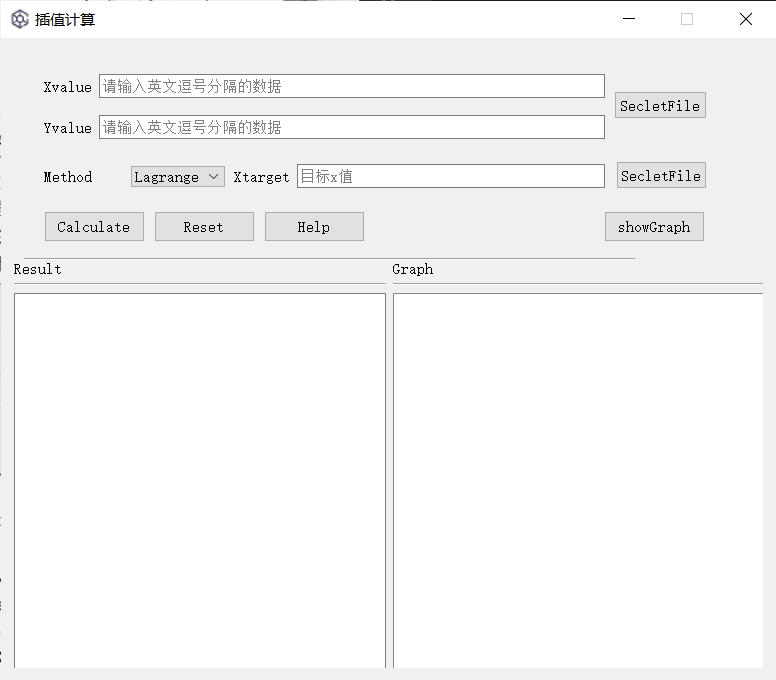
\includegraphics[scale= 0.4]{首页.png}
            }
            \hspace{0.1in}
            \subfigure[帮助界面]{
                \label{fig:help}
                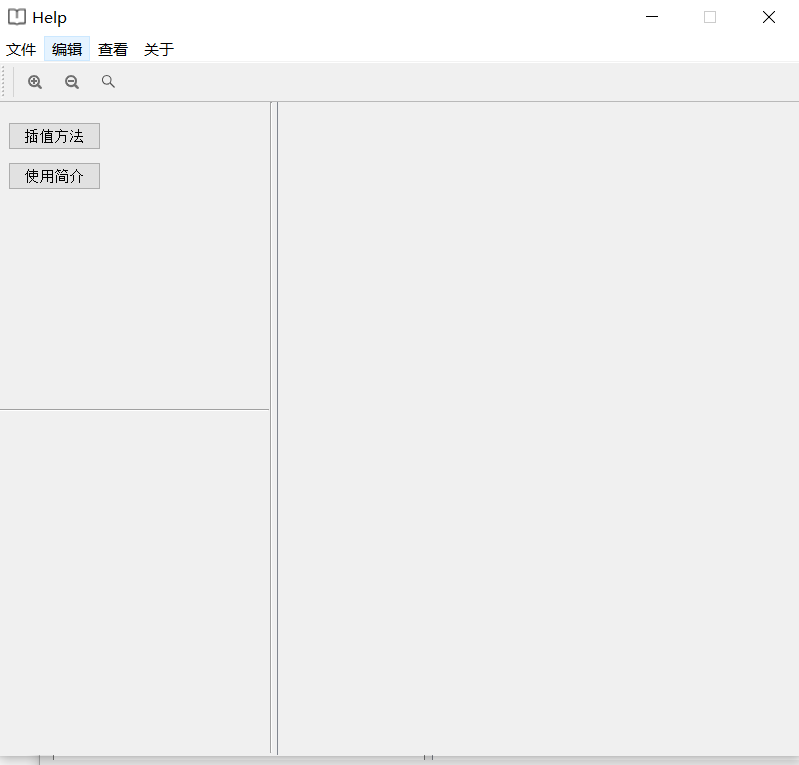
\includegraphics[scale= 0.4]{帮助.png}
            }
            \caption{软件界面}
            \label{fig:double}
        \end{figure}
        \begin{description}
            \item[数据输入] 用户输入以英文字符\emph{','}分隔的数据。
            也可以点击文件选项按钮选择指定格式的\emph{.csv}或者\emph{.txt}文件。
            需要注意的是文件需要以英文逗号分割,X数据和Y数据应该分别占一列。 
            \item[数据计算] 本软件提供“牛顿插值法”,“拉格朗日插值法”,“反插值法”,“三次样条插值”这四种方法。
            通过计算机模拟手动计算的过程来计算指定数据插值。 
            \item[结果演示] 通过matplotlib可视化作图来实现插值法的图形可视化,使得结果更加具有一般性和可行性,
            同时也加强了用户的软件使用体验。 
            \item[帮助文档] 本软件提供了帮助文档,通过点击“Help”按钮可以获得更加详细地使用说明和方法简介,
            同时也可以联系作者。 
        \end{description}    
        \subsection{插值方法部分}
            \begin{description}
                \item [牛顿插值法] 本方法默认采用基本的牛顿插商公式,通过计算机模拟查商表计算,取
                取插商表第一斜行的数据值进行计算。
                    \begin{figure}[htb]
                        \centering
                        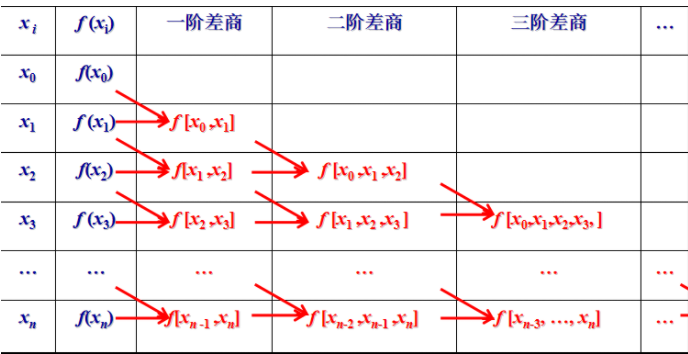
\includegraphics[scale = 0.6]{插商表.png}
                        \caption{插商表示意图}
                        \label{fig:newtontable}
                    \end{figure}
                \item [拉格朗日插值法] 本方法仍然采用计算机模拟手动计算的过程来实现。公式如下:
                    \begin{equation}
                        l_i(x) = \frac{(x-x_0)\dots(x-x_(i-1)(x-x_(i+1)\dots(x-x_n)}{(x_i-x_0)\dots(x_i-x_i-1)(x_i-x_i+1)\dots(x_i-x_n)}
                    \end{equation}
                    \begin{equation}
                        L_n(x) = \sum_{i=0}^n y_il_i(x)
                    \end{equation}
                \item [三次样条插值] 本方法融入了分段插值的思想,给定$n$个数据点,可以获得$n-1$段插值区间,
                在每一个插值区间内构造三次样条函数$ax^3+bx^2+cx+d$。
                构造方法具体如下,首先建立节点函数值相等的$n$个方程,
                然后建立首位端点的两个方程,
                再建立节点处一阶导数相等的$n$个方程,再是二阶导函数相等的$n$个方程,再是二阶导函数相等的,
                最后建设端点处的二阶导数为$0$构建$2$个方程。共计$2n+4$个方程。
                \item [反插值法] 这里我们采取简单的调换$x$和$y$值的方法快速实现,默认采用的是牛顿法。
            \end{description}
    \section{项目实现重点与细节}
        \subsection{界面实现}
            \paragraph{布局}
            本项目布局采用QTDesigner工具实现拖拽布局,利用PYUIC实现.ui文件转化为.py文件,从而实现窗口布局。
            如下图所示:
            \begin{figure}[htb]
                \centering
                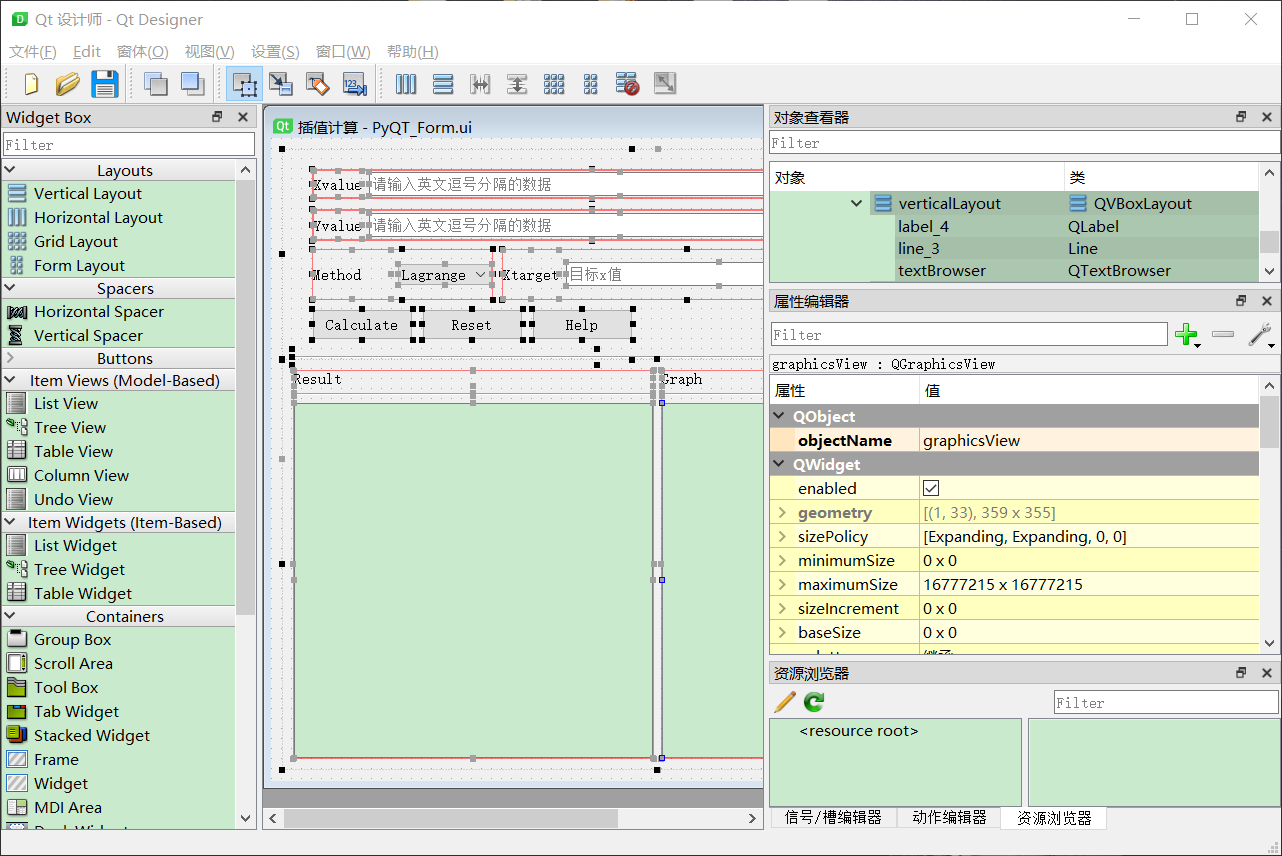
\includegraphics[scale = 0.4]{QTDesigner.png}
                \caption{QTDesiger}
                \label{fig:designer}
            \end{figure}
            \paragraph{输入格式限制}
            利用Python正则表达式来简单实现对于用户输入数据格式的限制(英文逗号分割的实数数据),符合格式则可以输入成功并且显示,反之则输入失败,
            且不会显示在输入框中,正则表达式如下:
            \begin{verbatim}
                reg = QRegExp('^(((-?\d+)(\.\d+)?),)+((-?\d+)(\.\d+))$')
                single_reg = QRegExp('^(-?\d+)(\.\d+)?$')
            \end{verbatim}
            同时支持通过选择指定格式的文件(.csv/.txt)来输入数据并且显示,如下图所示:
            \begin{figure}[htb]
                \centering
                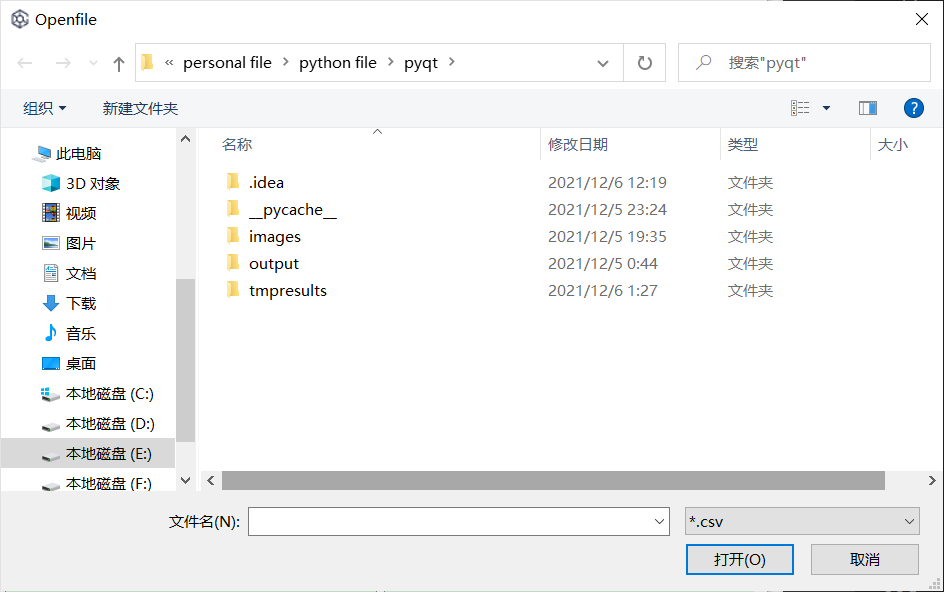
\includegraphics[scale = 0.4]{openfile.png}
                \caption{打开文件}
                \label{fig:openfile}
            \end{figure}
            \paragraph{Calculate的逻辑}
            这是一个重要的部分,用户点击计算按钮之后,程序会执行以下步骤,首先是判断是否有输入,然后是根据方法调用不同的api,
            随后再将结果显示在text-browser上,最后执行show-in-graph的绘图操作。操作结果如下图所示:
            \begin{figure}[htb]
                \centering
                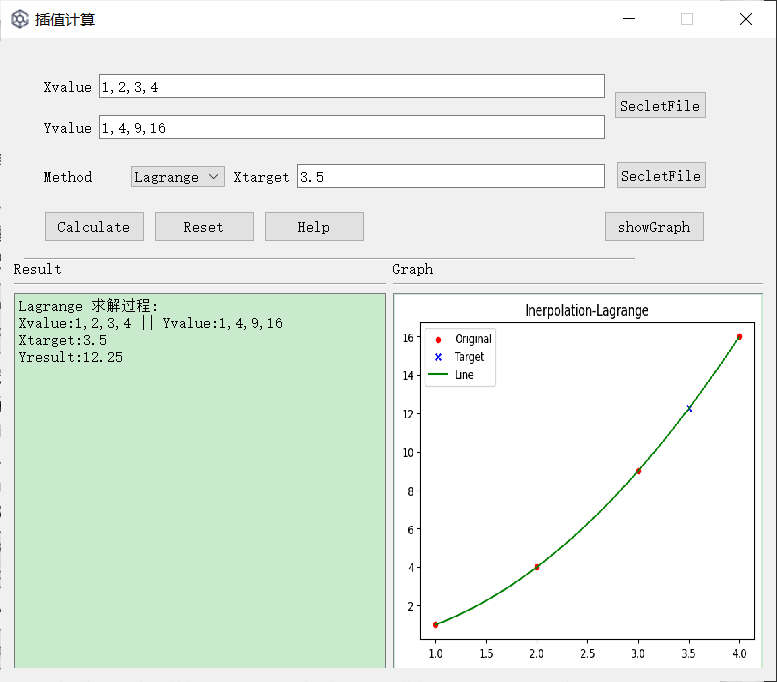
\includegraphics[scale = 0.5]{test.png}
                \caption{测试}
                \label{fig:test}
            \end{figure}
            \paragraph{显示}
            结果的文本显示,调用了self.textbrowser的api,结果的图形展示是调用了self.graphicsview的api将matplotlib的图集合到了软件里面。
        \subsection{插值实现}
            \subsubsection{牛顿插值法}
            计算机模拟手动求解插商表的关键核心代码是一条双重循环语句,如下:
            \begin{lstlisting}
                """从一阶差商开始一直到k阶差商"""
                for i in range(1, k + 1):
                """这是上一阶的插商,是计算这一阶插商的必要条件"""
                last_quotient = diff_quotient[i - 1] 
                tmp_quotient = []  # 初始化这一阶插商
                """遍历上一层差商的数值"""
                for j in range(0, len(last_quotient) - 1):
                    a = last_quotient[j]
                    b = last_quotient[j + 1]
                    """这里的索引需要仔细推敲"""
                    tmp_quotient.append((b - a) / (x_list[j + i] - x_list[j]))
                diff_quotient.append(tmp_quotient)
                """我们只需要这一阶插商的第一个数值 所以将他放入参数列表中"""
                parameters.append(tmp_quotient[0])  
            \end{lstlisting}
            \subsubsection{拉格朗日插值法}
            该方法的实现主要利用了numpy库的broadcast广播运算机制,利用concatenate函数方便地切片组合,其核心代码如下:
            \begin{lstlisting}
                upper = mul(x_target - np.concatenate((x_list[:i], x_list[i + 1:])))
                downer = mul(x0 - np.concatenate((x_list[:i], x_list[i + 1:])))
                result += upper / downer * y0
            \end{lstlisting}
            \subsubsection{三次样条插值}
            由于需要分段求解三次插值函数,并且每一段插值函数都存在许多的参数,实现过程较为复杂,具体处理步骤如下:
            \begin{lstlisting}
                def calcEquationPara()
                    """输入x_list,返回方程的系数,
                       返回形式是一个系数矩阵,按照降幂的方式排列
                    """
                def solutionOfEquation()
                    """输入x_list,y_list,返回每一段区间的三次函数的参数,降幂排列
                       获得方程解,然后计算机求解一个n元高次方程,
                       调用np.liag.solve(a, b)来解方程
                    """
                    """核心代码"""
                    while i < size_of_interval:  # 设置方程的右值
                        result[(i-1)*2] = y_list[i]
                        result[(i-1)*2+1] = y_list[i]
                        i += 1
                    result[(size_of_interval-1)*2] = y_list[0]
                    result[(size_of_interval-1)*2+1] = y_list[-1]
                    a = np.array(calcEquationPara(x_list))  # 获取方程左侧的系数矩阵
                    b = np.array(result)
                    return np.linalg.solve(a, b)  # 解方程
                def calculate()
                    """输入parameters和x值,返回插值计算的结果"""
            \end{lstlisting}
        \subsection{绘图实现与集成}
            \subsubsection{matplotlib绘图}
            通过matplotlib(Python语言优秀可视化第三方库)来对原始数据进行离散展示,特别标出目标点,并且绘制出一条完整的插值曲线
                \begin{lstlisting}
                    """核心代码"""
                    x = np.array(x, dtype=float)
                    x = np.append(x, target_x)
                    # 找到最大最小值求取x_range
                    min_x = x[np.argmin(x)]
                    max_x = x[np.argmax(x)]
                    x = np.delete(x, len(x)-1)
                    y = np.array(y, dtype=float)
                    target_x = float(target_x)
                    result = float(result)
                    plt.figure()
                    # 原始数据点
                    plt.scatter(x, y, c='r', marker='o', s=20, label='Original')
                    # 目标点
                    plt.scatter(target_x, result,c='b', marker='x', 
                        s=30, label='Target')
                    x_line = np.arange(min_x, max_x, (max_x - min_x) / 1000)
                    y_line = np.zeros(len(x_line))
                    # 函数拟合
                    plt.plot(x_line, y_line, c='g', label='Line')
                \end{lstlisting}
            \subsubsection{集成到软件}
            通过PyQT5的内置graphicsview模块来将已经生成好的matplotlib的.png文件格式显示到软件界面中,并且自动适应大小,
            软件体验更加完整。
                \begin{lstlisting}
                    # 获取文件路径
                    last_path = os.path.join(os.getcwd(), "tmpresults/" + 
                        str(self.cal_times) + ".png")
                    img = QPixmap()
                    img.load(last_path)
                    # 设置显示区域
                    self.graphicsView.scene = QGraphicsScene()
                    item = QGraphicsPixmapItem(img)
                    # 添加显示元素,这里就是图片
                    self.graphicsView.scene.addItem(item)
                    self.graphicsView.setScene(self.graphicsView.scene)
                    #图片自适应view栏的大小
                    self.graphicsView.fitInView(QGraphicsPixmapItem(img))
                \end{lstlisting}
    \section{项目特点}
        \paragraph{优秀的用户体验} 软件具有良好的用户反馈,包括成功提示,错误提示,未选择提示,
        输入检验等效果如下图所示:
        \begin{figure}[htb]
            \centering
            \subfigure[输入反馈]{
                 \label{fig:inputerror}
                 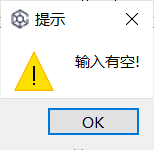
\includegraphics[scale= 0.6]{inputerror.png}
            }
            \hspace{2em}
            \subfigure[关于作者]{
                \label{fig:about}
                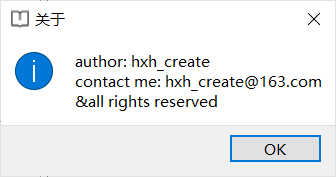
\includegraphics[scale=0.6]{about.png}
            } 
            \hspace{2em}
            \subfigure[文件反馈]{
                \label{fig:fileerror}
                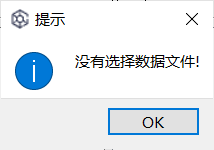
\includegraphics[scale=0.6]{fileerror.png}
            }
            \caption{用户体验}
            \label{fig:trible}
        \end{figure}
        \paragraph{支持帮助文档} 软件提供内嵌式的帮助说明文档可以更加有效地帮助用户使用该工具,了解该工具的实现原理等
        \paragraph{资源占用} 所有产生的数据文件,图片文件都将存储在tmpresults文件夹里面,当点击软件关闭的同时,会清楚该文件夹的所有内容,
        减少资源的占用,提升该工具的运行程序,避免了大量数据的堆积。
        \paragraph{计算的鲁棒性} 本工具在做插值计算的时候特别针对程序进行了鲁棒性的优化。
            \begin{itemize}
                \item 第一点是用户的xlist和ylist的输入不需要按照一定的顺序,程序会自动进行一个排序之后再进行插值处理。
                \item 是用户的target目标值并不需要处于xlist或者ylist的范围,仍然能够完成运算。
                        因为我们插值实现的过程中是采用了原始的插商表或者插值公式
                        进行计算的。(三次样条插值由于其实现的局限性,目标值必须出现在范围内,否则无法进行计算)
                \item 第三点在于数据支持多种类型。整数支持达到32位,小数的支持达到小数点后17位,几乎覆盖了日常的所有计算需求。
            \end{itemize}
    \section{体会与总结}
        \begin{enumerate}
            \item 学习了Python的GUI编程的基本知识,对软件开发流程有了基本的熟悉与了解。
            \item 通过大量资料的查询也对插值法的各大语言和库的优秀实现方法做了一个了解。
            \item 从理论层面的数值分析课程中跳出来,结合编程知识对已经掌握的知识进行了编程的实现,对于插值法有了更为深入的理解。
            
        \end{enumerate}
    \section{附录}
        \subsection{软件程序源码及可执行文件}
        \href{https://gitee.com/hxh_create/numerical-analysis-operation}{点击跳转gitee}
        
        \href{https://github.com/hxhcreate/numerical-analysis-work/tree/master}{点击跳转github}
    \bibliography{math}
\end{document}